\scanpage{31}

Supposons $j$ et $j'$ ainsi choisis. Si $j,j'$ sont injectifs, on en déduit une biextension
\inserted{\rlap{\raisebox{.4ex}{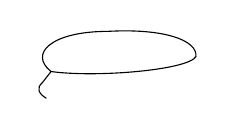
\begin{tikzpicture}[baseline]\draw (.14,-.21) .. controls (-.15,.02) and (.15,.30) .. (.86,.30) .. controls (1.57,.34) and (2.00,.19) .. (1.98,-.02) .. controls (1.88,-.19) and (.72,-.29) .. (.14,-.21) -- (.03,-.35) .. controls (-.05,-.42) and (-.02,-.49) .. (.08,-.55);\end{tikzpicture}}}canonique}
\deleted{\unsure{de|des}} $(A,A')$, où $A=G/M$, $A'=G'/M'$. Dans le cas général, posons

\deleted{\unsure{p\textsuperscript{r}|ps} \unsure{dire|dis} qu'on a une biextension de}
\[
A=\left[\underset{\text{deg.}\,\unsure{<|-}1}{M}\longrightarrow\underset{\text{deg}\,0}{G}\right],\qquad
A'=\left[M'\unsure{\longrightarrow|\mathbin{-}}G'\right].
\]

d'où
\diagram{\begin{tabular}{@{}c@{\quad}c@{\quad}c@{}}
\begin{tikzcd}[ampersand replacement=\&,row sep=small,column sep=small]
 \& \& A \arrow[dl,"1"'] \& \& \\
 \unsure{\leftarrow|\mathbin{-}} \& M \arrow[rr,"{\begin{tikzpicture}[baseline,x=1em,y=1em]\draw[line width=.4pt] (-.38,-.3)--(.38,-.3);\end{tikzpicture}}"{description,pos=.30,inner sep=0pt,fill=none}] \& \& G \arrow[ul] \arrow[r,no head] \& \phantom{0}
\end{tikzcd}
&
\begin{minipage}{2.5cm}\centering\unsure{complexe} de\par\unsure{faisceaux|chaînes} ?\end{minipage}
&
\begin{tikzcd}[ampersand replacement=\&,row sep=small,column sep=small]
 \& \& A' \arrow[dl,"1"'] \& \\
 \phantom{0} \& M' \arrow[l] \arrow[rr,no head] \& \& G' \arrow[ul]
\end{tikzcd}
\end{tabular}}

on \unsure{va|en} \unsure{définir|définit} une \deleted{\unsure{biextension}} classe canonique
\[
\xi\in\operatorname{Ext}^1(A\mathbin{\overset{L}{\otimes}}A',G_m),
\]

\margin{\unsure{pour ainsi dire|pourquoi} ?}
\noindent\llap{\raisebox{-2.65cm}[0pt][0pt]{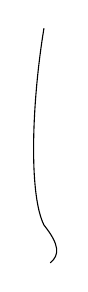
\begin{tikzpicture}\draw (0,2.8) .. controls (-.15,1.9) and (-.2,.7) .. (0,.3) .. controls (.2,.05) and (.2,-.08) .. (.08,-.18);\end{tikzpicture}}\hspace{.7em}}%
\begin{minipage}[t][3cm][t]{\linewidth}
jouant le rôle d'une biextension de $(A,A')$ par $G_m$.

\medskip
Soit en effet \textendash\,\textendash\,\textendash\,\textemdash\,\textendash
\end{minipage}

\unsure{Soit|Soient}
\[
{}_nA\overset{\text{\unsure{dfn|def}}}{=}\deleted{\unsure{R}}\underline{\operatorname{Ext}}^0(\mathbb Z/n\mathbb Z,A),\qquad
{}_nA'=\operatorname{\underline{Ex}t}^0(\mathbb Z/n\mathbb Z,A')
\]
on trouve, \unsure{que|qu'on}, grâce aux \unsure{triangle|triangles} plus haut,
\margin{\deleted{\uline{\unsure{Soit}}}}
\[
\left\{\begin{aligned}
{}_nM&=0\quad
\overset{\text{\inserted{\rlap{\raisebox{.25ex}{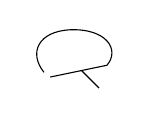
\begin{tikzpicture}[baseline]\draw (.02,-.22) .. controls (-.18,.03) and (-.05,.30) .. (.35,.32) .. controls (.81,.34) and (.99,.07) .. (.82,-.13) -- (.10,-.28);\draw (.50,-.20)--(.72,-.42);\end{tikzpicture}}}\unsure{resp.|pq}}}}{\deleted{{}_nM'=0}}\\
nG&=G\quad\text{p.ex}\quad\text{\deleted{\unsure{par}}}\ nB=B,\ nT=T\quad(\text{ce dernier résulte de }{}_nM=0
\end{aligned}\right.
\]

\margin{\begin{minipage}[t]{1.85cm}donne aussi autre \unsure{interprét\textsuperscript{tion}|interpr.\textsuperscript{tion}} de $ {}_nA$, via hom. cobord si $nG=G$\end{minipage}\hspace{.15cm}\begin{tikzpicture}[baseline]\draw (0,-2.5)--(0,0);\end{tikzpicture}}
\diagram{\begin{tikzcd}[ampersand replacement=\&,column sep=small]
0 \arrow[r] \& \underset{\makebox[0pt][l]{\begin{tikzpicture}[overlay,baseline,x=1em,y=1ex]\draw (.55,1.7) .. controls (.45,2.6) and (1.45,2.2) .. (2.10,2.4) .. controls (2.32,2.45) and (2.40,3.4) .. (2.55,3.7) .. controls (2.70,2.8) and (3.15,2.1) .. (4.30,2.2) .. controls (4.8,2.3) and (5.20,2.1) .. (5.35,1.5);\end{tikzpicture}}(D(\unsure{M'_n|M_n}),\unsure{nB|{}_nB}),\,\text{si }nT=T}{ {}_nG} \arrow[r] \& {}_nA \arrow[r] \& M_n \arrow[r] \& 0
\end{tikzcd}}

et on a de $\widehat{\mathrm m}$ une suite exacte
\diagram{\begin{tikzcd}[ampersand replacement=\&,column sep=small]
0 \arrow[r] \& {}_n\unsure{G'|C'} \arrow[r] \& {}_nA' \arrow[r] \& M'_n \arrow[r] \& 0
\end{tikzcd}}

sous les hyp. duales; \unsure{passant|passons} à la limite sur $n=\ell^\nu$, \unsure{on a|on les}
\[
\vcenter{\hbox{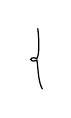
\begin{tikzpicture}[x=1em,y=1em]\draw[line width=.45pt] (.22,2.20) .. controls (.27,1.85) and (.29,1.25) .. (.19,1.11) .. controls (-.12,1.22) and (-.10,.92) .. (.19,1.05) .. controls (.24,.80) and (.22,.30) .. (.39,0);\end{tikzpicture}}}\,\begin{gathered}
\begin{tikzcd}[ampersand replacement=\&,column sep=small]
0 \arrow[r] \& T_\ell(G) \arrow[r] \& T_\ell(A) \arrow[r] \& M\otimes\mathbb Z_\ell \arrow[r,no head] \& 0
\end{tikzcd}\\
\begin{tikzcd}[ampersand replacement=\&,column sep=small]
0 \arrow[r,no head] \& T_\ell(A') \arrow[r] \& T_\ell(A') \arrow[r,no head] \& M'\otimes\mathbb Z_\ell \arrow[r] \& 0
\end{tikzcd}
\end{gathered}
\]
\margin{30}

